%%%%%%%%%%%%%%%%%%%%%%%%%%%%%%%%%%%%%%%%%
% Beamer Presentation
% LaTeX Template
% Version 2.0 (March 8, 2022)
%
% This template originates from:
% https://www.LaTeXTemplates.com
%
% Author:
% Vel (vel@latextemplates.com)
%
% License:
% CC BY-NC-SA 4.0 (https://creativecommons.org/licenses/by-nc-sa/4.0/)
%
%%%%%%%%%%%%%%%%%%%%%%%%%%%%%%%%%%%%%%%%%

%----------------------------------------------------------------------------------------
%	PACKAGES AND OTHER DOCUMENT CONFIGURATIONS
%----------------------------------------------------------------------------------------
\documentclass[
  24pt, % Set the default font size, options include: 8pt, 9pt, 10pt, 11pt, 12pt, 14pt, 17pt, 20pt
  %t, % Uncomment to vertically align all slide content to the top of the slide, rather than the default centered
  aspectratio=169, % Uncomment to set the aspect ratio to a 16:9 ratio which matches the aspect ratio of 1080p and 4K screens and projectors
]{beamer}

\graphicspath{{Images/}{./}} % Specifies where to look for included images (trailing slash required)

\usepackage{booktabs} % Allows the use of \toprule, \midrule and \bottomrule for better rules in tables

%----------------------------------------------------------------------------------------
%	SELECT LAYOUT THEME
%----------------------------------------------------------------------------------------

% Beamer comes with a number of default layout themes which change the colors and layouts of slides. Below is a list of all themes available, uncomment each in turn to see what they look like.

%\usetheme{default}
%\usetheme{AnnArbor}
%\usetheme{Antibes}
%\usetheme{Bergen}
%\usetheme{Berkeley}
%\usetheme{Berlin}
\usetheme{Boadilla} %me gusta
%\usetheme{CambridgeUS}
%\usetheme{Copenhagen}
%\usetheme{Darmstadt}
%\usetheme{Dresden}
%\usetheme{Frankfurt}
%\usetheme{Goettingen} %dos dos
%\usetheme{Hannover} %dos dos
%\usetheme{Ilmenau}
%\usetheme{JuanLesPins}
%\usetheme{Luebeck}
%\usetheme{Madrid}
%\usetheme{Malmoe}
%\usetheme{Marburg}
%\usetheme{Montpellier}
%\usetheme{PaloAlto}
%\usetheme{Pittsburgh}
%\usetheme{Rochester} %muy flat
%\usetheme{Singapore}
%\usetheme{Szeged}
%\usetheme{Warsaw}

%----------------------------------------------------------------------------------------
%	SELECT COLOR THEME
%----------------------------------------------------------------------------------------

% Beamer comes with a number of color themes that can be applied to any layout theme to change its colors. Uncomment each of these in turn to see how they change the colors of your selected layout theme.

%\usecolortheme{albatross}
%\usecolortheme{beaver}
%\usecolortheme{beetle}
%\usecolortheme{crane}
%\usecolortheme{dolphin}
%\usecolortheme{dove}
%\usecolortheme{fly}
%\usecolortheme{lily} %default
%\usecolortheme{monarca}
%\usecolortheme{seagull}
%\usecolortheme{seahorse}
%\usecolortheme{spruce}
%\usecolortheme{whale}
%\usecolortheme{wolverine}

%----------------------------------------------------------------------------------------
%	SELECT FONT THEME & FONTS
%----------------------------------------------------------------------------------------

% Beamer comes with several font themes to easily change the fonts used in various parts of the presentation. Review the comments beside each one to decide if you would like to use it. Note that additional options can be specified for several of these font themes, consult the beamer documentation for more information.

\usefonttheme{default} % Typeset using the default sans serif font
%\usefonttheme{serif} % Typeset using the default serif font (make sure a sans font isn't being set as the default font if you use this option!)
%\usefonttheme{structurebold} % Typeset important structure text (titles, headlines, footlines, sidebar, etc) in bold
%\usefonttheme{structureitalicserif} % Typeset important structure text (titles, headlines, footlines, sidebar, etc) in italic serif
%\usefonttheme{structuresmallcapsserif} % Typeset important structure text (titles, headlines, footlines, sidebar, etc) in small caps serif

%------------------------------------------------

%\usepackage{mathptmx} % Use the Times font for serif text
\usepackage{palatino} % Use the Palatino font for serif text

\usepackage[ruled,vlined]{algorithm2e}
%\usepackage{helvet} % Use the Helvetica font for sans serif text
\usepackage[default]{opensans} % Use the Open Sans font for sans serif text
\usepackage[spanish]{babel}
\usepackage{dirtree}
\usepackage{xcolor}
%\usepackage[default]{FiraSans} % Use the Fira Sans font for sans serif text
%\usepackage[default]{lato} % Use the Lato font for sans serif text

\usepackage[scaled]{helvet}
\usepackage[round]{natbib}
%\newcommand{\newblock}{}

\usepackage{rotating}

\newcommand\FourQuad[4]{%
  \begin{minipage}[b][.33\textheight][t] 
    {.48\textwidth}#1\end{minipage}\hfill%
    \begin{minipage}[b][.33\textheight][t] 
      {.48\textwidth}#2\end{minipage}\\[0.5em]
      \begin{minipage}[b][.33\textheight][t] 
        {.48\textwidth}#3\end{minipage}\hfill
        \begin{minipage}[b][.33\textheight][t] 
          {.48\textwidth}#4\end{minipage}%
}

\usepackage{tikz}
%\usetikzlibrary{arrows,shapes,positioning,shadows,trees,quotes}


%\tikzset{
%  basic/.style  = {draw, text width=2cm, drop shadow, font=\sffamily, rectangle},
%  root/.style   = {basic, rounded corners=2pt, thin, align=center,
%                   fill=green!30},
%  level 2/.style = {basic, rounded corners=6pt, thin,align=center, fill=green!60,
%                   text width=8em},
%  level 3/.style = {basic, thin, align=left, fill=pink!60, text width=6.5em}
%}

\usetikzlibrary{calc}

\tikzstyle{part} = [rectangle, rounded corners, minimum width=3cm, minimum height=1cm,     align=center, draw=black]
\tikzstyle{chapter} = [rectangle, rounded corners, minimum width=3cm, minimum height=1cm,     align=center, draw=black, text width=3.5cm]
\tikzstyle{arrow} = [thick, ->]

\usepackage{array} % needed for \arraybackslash
\usepackage{graphicx}
\usepackage{adjustbox} % for \adjincludegraphics

\usepackage{subcaption}
\usepackage{bibentry}
%\bibliographystyle{apalike}
\usepackage{chngcntr}
\usepackage{lipsum}% http://ctan.org/pkg/lipsum
\usepackage{hanging}% http://ctan.org/pkg/hanging

\usepackage{xcolor,colortbl}
\usepackage{multirow}

\usepackage{animate}
\usepackage{multicol}
\usepackage{tabularx,booktabs}
\usepackage{forloop}
\usepackage{ragged2e}

\usepackage{bbding} %palomitas checkmark
\usepackage{pifont}
\usepackage{lipsum,tabularx}
\newcounter{loopcntr}

%----------------------------------------------------------------------------------------
%	SELECT INNER THEME
%----------------------------------------------------------------------------------------

% Inner themes change the styling of internal slide elements, for example: bullet points, blocks, bibliography entries, title pages, theorems, etc. Uncomment each theme in turn to see what changes it makes to your presentation.

\useinnertheme{circles}

%----------------------------------------------------------------------------------------
%	SELECT OUTER THEME
%----------------------------------------------------------------------------------------

% Outer themes change the overall layout of slides, such as: header and footer lines, sidebars and slide titles. Uncomment each theme in turn to see what changes it makes to your presentation.

\setbeamertemplate{footline}[frame number] % Uncomment this line to replace the footer line in all slides with a simple slide count
\setbeamertemplate{navigation symbols}{} % Uncomment this line to remove the navigation symbols from the bottom of all slides

%----------------------------------------------------------------------------------------
%	PRESENTATION INFORMATION
%----------------------------------------------------------------------------------------

\title[PROTOCOLO DE INVESTIGACIÓN]{%\centering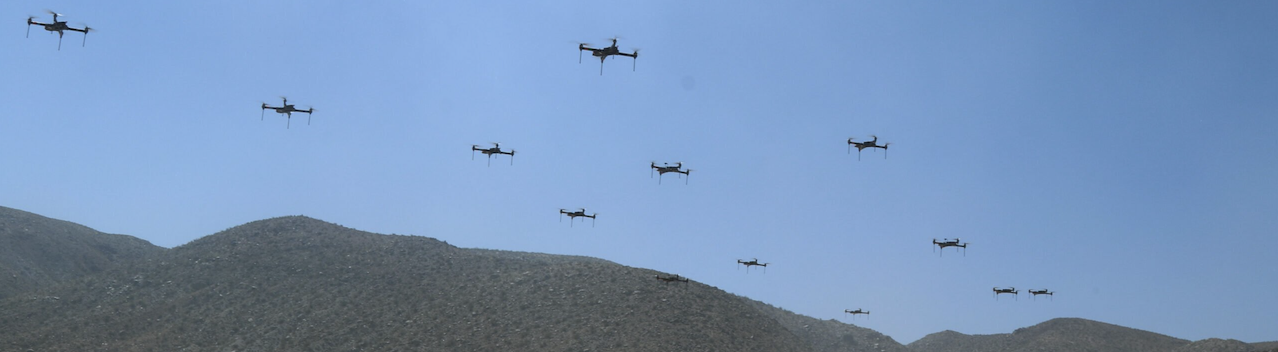
\includegraphics[width=10cm]{swarm_drones}\\
  Estrategias para la exploración coordinada multi-VANT} % The short title in the optional parameter appears at the bottom of every slide, the full title in the main parameter is only on the title page

%\subtitle{Optional Subtitle} % Presentation subtitle, remove this command if a subtitle isn't required

\author[]{Luis Alberto Ballado Aradias\\[\baselineskip]
  \small{{Asesores:} \\
    \and\\Dr. José Gabriel Ramírez-Torres
    \and\\Dr. Eduardo Rodriguez-Tello }}

\institute[CINVESTAV]{
  CINVESTAV UNIDAD TAMAULIPAS \\
  %\smallskip \textit{luis.ballado@cinvestav.mx}
} % Your institution, the optional parameter can be used for the institution shorthand and will appear on the bottom of every slide after author names, while the required parameter is used on the title slide and can include your email address or additional information on separate lines


\date[\today]{Cd. Victoria, Tamaulipas - \today} % Presentation date or conference/meeting name, the optional parameter can contain a shortened version to appear on the bottom of every slide, while the required parameter value is output to the title slide

%\titlegraphic{\hspace*{8.75cm}~%
%   
\includegraphics[width=0.8cm]{cinvestavlogo}
%}

%----------------------------------------------------------------------------------------

\counterwithin*{footnote}{page}
\newcommand\footcite[1]{\footnote{\bibentry{#1}}\label{\thepage:#1}}
\newcommand\secondcite[1]{\textsuperscript{\ref{\thepage:#1}}}

\newcommand{\rpt}[2][1]{%
  \forloop{loopcntr}{0}{\value{loopcntr}<#1}{#2}%
}
\newcommand{\on}[1][1]{
  \forloop{loopcntr}{0}{\value{loopcntr}<#1}{&\cellcolor{gray}}
}
\newcommand{\onok}[1][1]{
  \forloop{loopcntr}{0}{\value{loopcntr}<#1}{&\cellcolor{green}}
}
\newcommand{\off}[1][1]{
  \forloop{loopcntr}{0}{\value{loopcntr}<#1}{&\cellcolor{white}}
}

\addtolength{\textheight}{90pt}

\newcommand{\I}{\mathbb{I}}
\newcommand{\K}{\mathbb{K}}
\newcommand{\N}{\mathbb{N}}
\newcommand{\Q}{\mathbb{Q}}
\newcommand{\R}{\mathbb{R}}
\newcommand{\Z}{\mathbb{Z}}

\newcommand{\specialcell}[2][c]{%
  \begin{tabular}[#1]{@{}c@{}}#2\end{tabular}}


\begin{document}

%----------------------------------------------------------------------------------------
%	TITLE SLIDE
%----------------------------------------------------------------------------------------

\begin{frame}
  \titlepage % Output the title slide, automatically created using the text entered in the PRESENTATION INFORMATION block above
\end{frame}

%----------------------------------------------------------------------------------------
%	TABLE OF CONTENTS SLIDE
%----------------------------------------------------------------------------------------

% The table of contents outputs the sections and subsections that appear in your presentation, specified with the standard \section and \subsection commands. You may either display all sections and subsections on one slide with \tableofcontents, or display each section at a time on subsequent slides with \tableofcontents[pausesections]. The latter is useful if you want to step through each section and mention what you will discuss.
\AtBeginSection[]
{
  \begin{frame}
    \frametitle{Contenido} % Slide title, remove this command for no title
    \tableofcontents[currentsection] % Output the table of contents (all sections on one slide)
    %\tableofcontents[pausesections] % Output the table of contents (break sections up across separate slides)
  \end{frame}
}

\pretocmd{\tableofcontents}{\thispagestyle{empty}}{}{}

%----------------------------------------------------------------------------------------
%	PRESENTATION BODY SLIDES
%----------------------------------------------------------------------------------------

\section{Resumen}
\begin{frame}{Resumen}
  \bigskip % Vertical whitespace
  \centering
  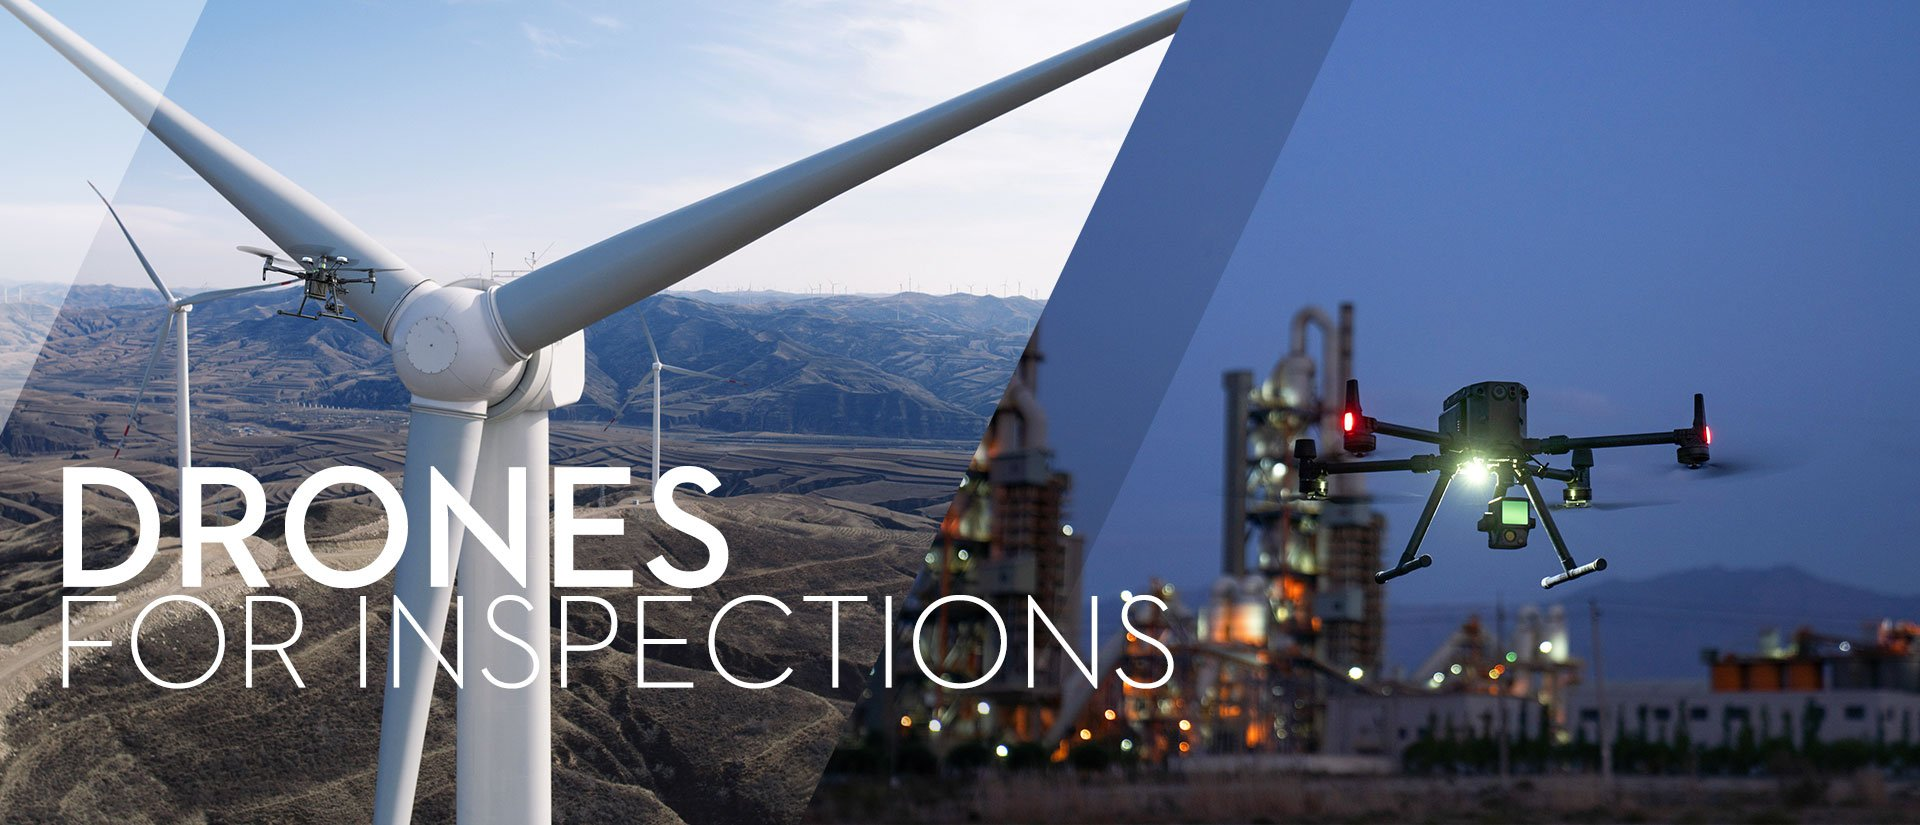
\includegraphics[width=0.45\textwidth,height=0.35\textheight]{DJI_B1}$^\dag$
  \hfil
  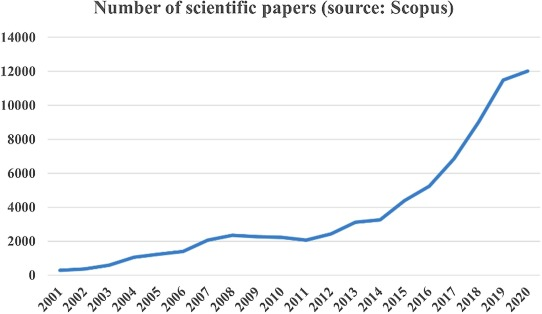
\includegraphics[width=0.45\textwidth,height=0.35\textheight]{survey_chart.jpg}\footnotemark
  \vspace{2pt}\\
  
  \begin{itemize}
  \item \textbf{Aplicaciones} en lugares inaccesibles o peligrosos.
  \item \textbf{Múltiples VANT} pueden reducir el tiempo de exploración y aumentar la confianza del sistema.
  \item \textbf{Limitaciones} en carga, procesamiento y batería influyen en el tiempo de vuelo.
  \end{itemize}

  \footnotetext{UAV in the advent of the twenties: Where we stand and what is next [\cite{Nex2022}]}
  %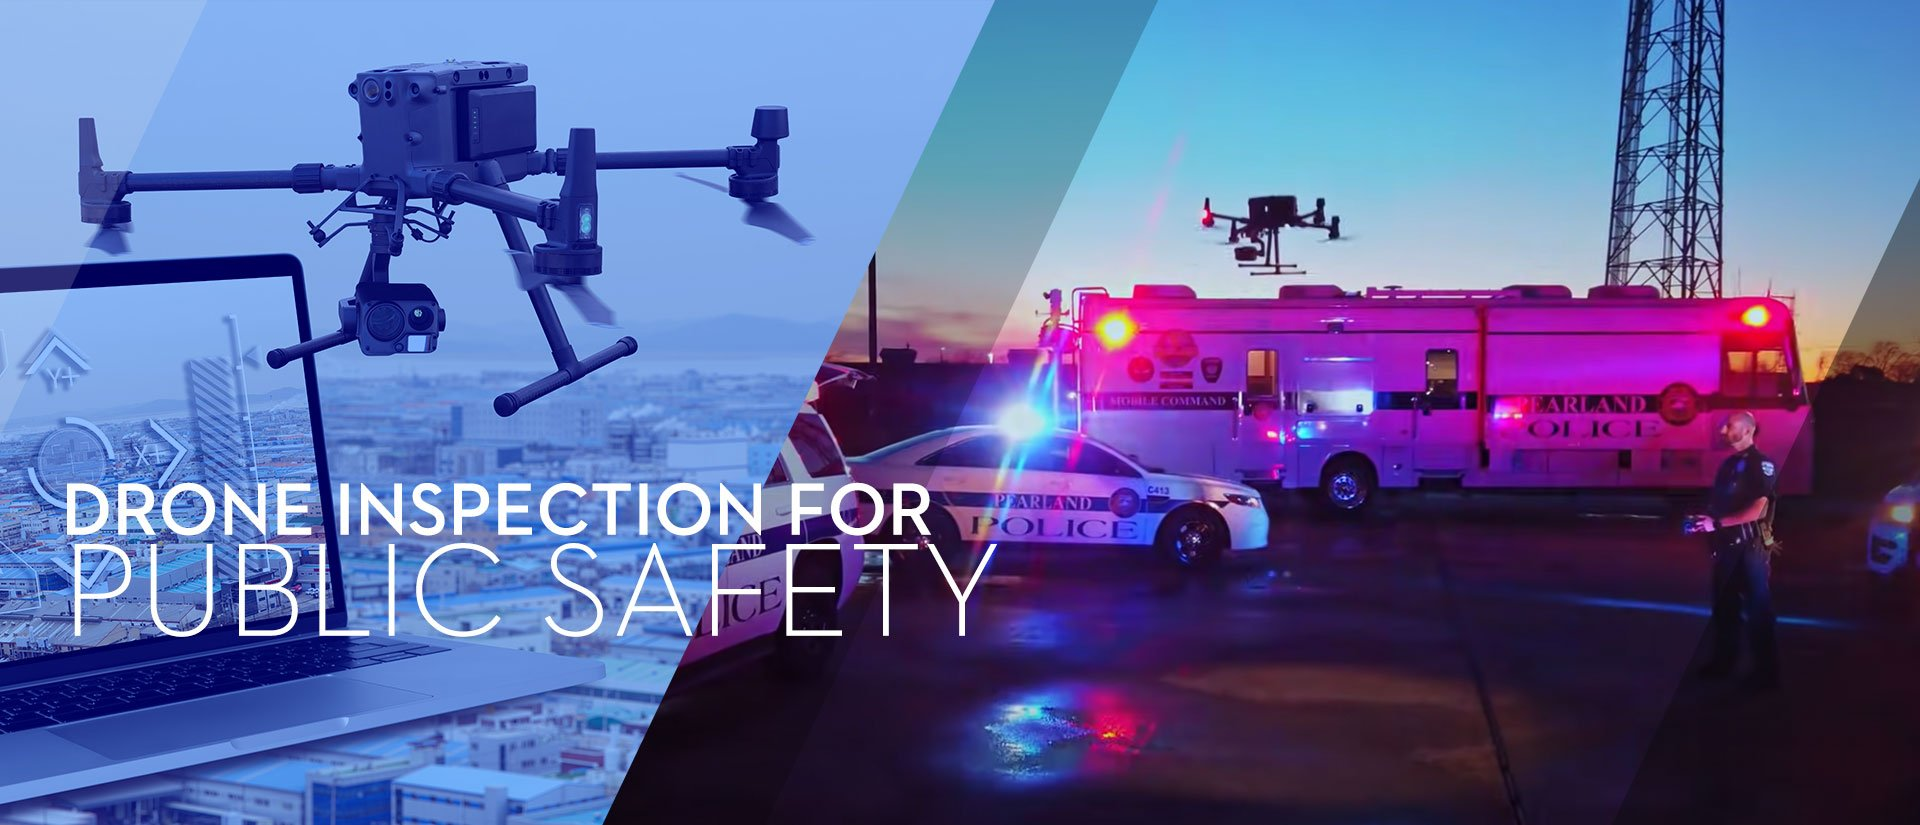
\includegraphics[width=0.45\textwidth,height=0.35\textheight]{DJI_B5}$^\dag$ 
  %\hfil
  %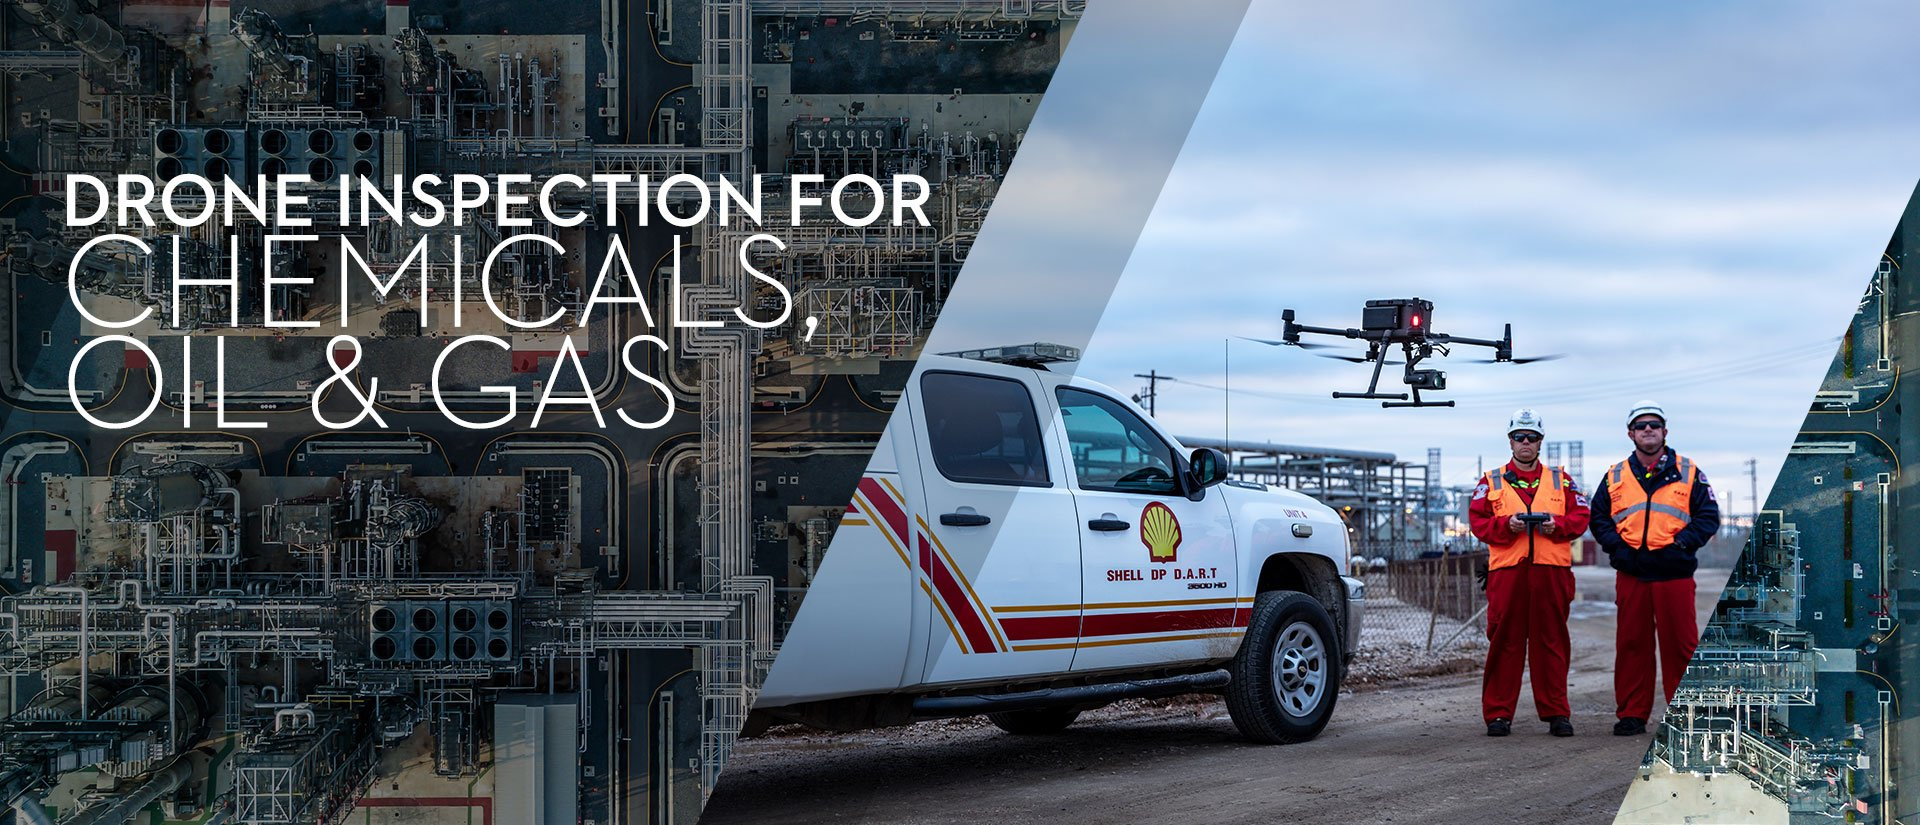
\includegraphics[width=0.45\textwidth,height=0.35\textheight]{DJI_B4}$^\dag$\\
  %\rule{0in}{1.2em}$^\dag$ \small Inspecciones con VANT basadas en los mejores casos de uso\\
  %\tiny \url{https://enterprise-insights.dji.com/blog/complete-guide-to-drone-inspections}
\end{frame}

\section{Robot Autónomo}
\begin{frame}
  \frametitle{Robot Autónomo}

  \centering
  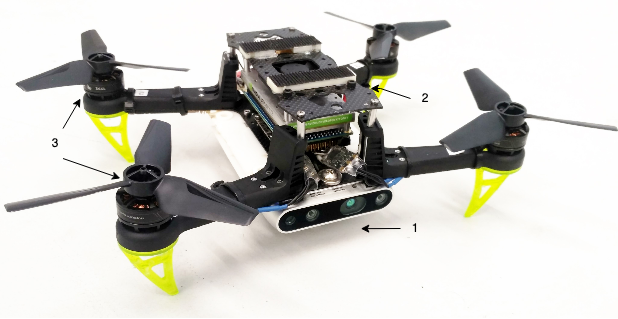
\includegraphics[width=8cm]{drone_taxo}
  \bigskip % Vertical whitespace
  \begin{itemize}
  \item \textbf{1.- \underline{Percepción -}} Incluyen cámaras de profundidad, sensores tipo LiDAR, entre otros. Permiten al VANT recopilar información sobre su entorno.
  \item \textbf{2.- \underline{Control -}} Computadora a bordo, contiene el poder computacional para la toma de decisiones autónomas basada en la información recopilada por los sensores.
  \item \textbf{3.- \underline{Actuadores -}} Motores y hélices que proporcionan la fuerza necesaria para el vuelo.
  \end{itemize}
\end{frame}

\begin{frame}{Control de un VANT}

  \begin{minipage}{0.47\textwidth}
    
    \small UN blah blah ...
    
    \begin{itemize}
    \item item
    \item item
    \item item
    \item item
    \end{itemize}
  \end{minipage}
  \hspace{0.2cm}
  \begin{minipage}{0.5\textwidth}
    \centering
    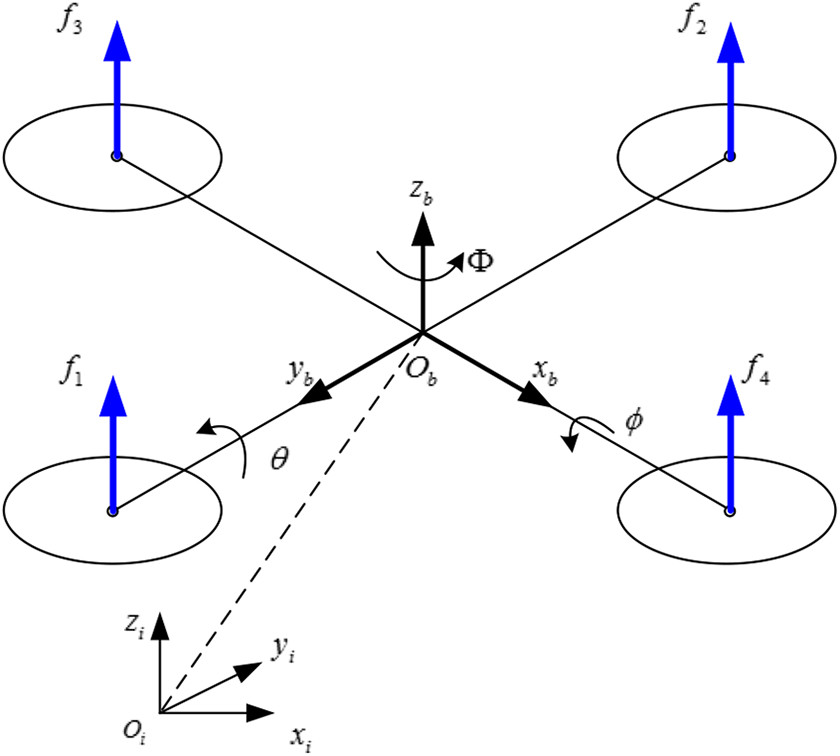
\includegraphics[width=4cm]{uav_model.jpeg}
    \bigskip % Vertical whitespace
  \end{minipage}
\end{frame}

\begin{frame}  
  %\centering
  Principales preguntas que un robot autónomo debe responder \footnotemark
  \bigskip % Vertical whitespace
  \begin{itemize}
  \item \textcolor{blue}{¿Dónde estoy?} $\implies$ Localización y representación del medio ambiente \pause 
  \item \textcolor{blue}{¿A dónde voy?} $\implies$ Toma de decisiones \pause  %Cognición
  \item \textcolor{blue}{¿Cómo llego hasta ahí?} $\implies$ Planificación de trayectoria 
  \end{itemize}
  \pause
  \bigskip % Vertical whitespace

  \begin{minipage}{0.47\textwidth}
    Para resolver estas preguntas,\\
    el robot debe: 
    
    \begin{itemize}
    \item Tener un modelo del ambiente (dado, o autónomamente construido)
    \item Localizarse dentro del ambiente
    \item Planear y ejecutar los movimientos
    \end{itemize}
    
    \footnotetext{Visual map making for a mobile robot [\cite{1087348}]}
  \end{minipage}
  \hspace{0.2cm}
  \begin{minipage}{0.5\textwidth}
    \centering
    \animategraphics[loop,width=8cm]{10}{ezgif-frame-}{001}{130}
    \rule{0in}{1.2em}$^\dag$\scriptsize Indoor Autonomous UAV Exploration Planning.\\
    \tiny \url{https://www.youtube.com/watch?v=oVOU8EDsWrM} 
  \end{minipage}
\end{frame}

\begin{frame}{Localización - ¿Dónde estoy?}

  Problema de Localización y Mapeo Simultáneos  \footnote{Simultaneous localization and mapping: part I [\cite{slam_doc}]}
  \bigskip % Vertical whitespace
  \begin{itemize} 
    \item \textcolor{blue}{VER}: El Robot utiliza la lectura de sus sensores para encontrarse a el mismo.
      \bigskip % Vertical whitespace
    \item \textcolor{red}{ACTUAR}: El Robot, se mueve hacia adelante
      \begin{itemize}
      \item Movimiento estimado a partir de las lecturas de la odometría.
      \item Acumulación de incertidumbre.
      \end{itemize}
      \bigskip % Vertical whitespace
    \item \textcolor{blue}{VER}: Lectura de sus sensores nuevamente para localizarse a sí mismo
  \end{itemize}
      
  \bigskip % Vertical whitespace
  Belief update (Actualización de creencia) \footnote{Uncertain geometry in robotics [\cite{slam_dur}]} \footnote{Estimating Uncertain Spatial Relationships in Robotics [\cite{Smith1988}]}
  
\end{frame}

\begin{frame}{Formulación del Problema de Localización y Mapeo Simultáneos}

  Dados:
  \begin{itemize}
  \item Conjunto de observaciones $z = \{z_1,z_2,...,z_t\}$
  \item Conjunto de comandos de control $u = \{u_1,u_2,...,u_t\}$
  \end{itemize}
  \bigskip % Vertical whitespace
  Requerimos:
  \begin{itemize}
  \item Mapa del ambiente $m$
  \item Trayectoria del robot $x = \{x_1,x_2,...,x_t\}$
  \end{itemize}
  \bigskip % Vertical whitespace
  
  En terminos probabilisticos: Estimar la trayectoria del robot y el mapa

  \centering
  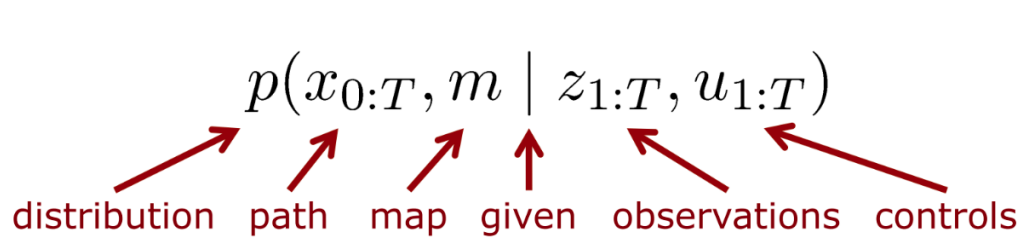
\includegraphics[width=8cm]{slam1}
  
\end{frame}

\begin{frame}{Formulación del Problema de Localización y Mapeo Simultáneos}

  \begin{itemize}
  \item La trayectoria del robot y el mapa son desconocidos.
  \item Correlación entre el mapa y las posiciones del robot. 
  \end{itemize}

  \centering

  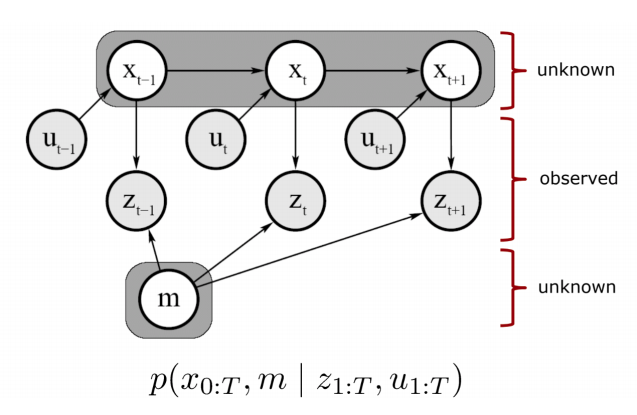
\includegraphics[width=8cm]{slam2}

\end{frame}

\begin{frame}{Modelos de observación y posición}

  \centering

  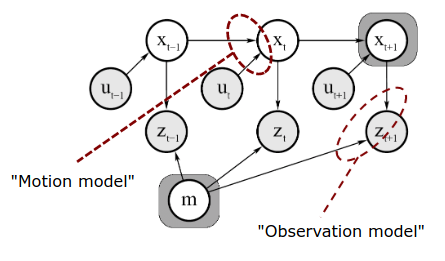
\includegraphics[width=8cm]{slam3}

\end{frame}

\begin{frame}{Modelos}

  \centering

  \begin{itemize}
  \item Observación\\
    
\includegraphics[width=8cm]{slam5}  
  \item Posición\\
    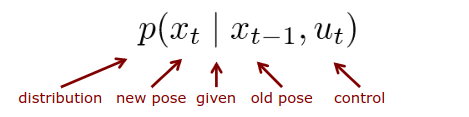
\includegraphics[width=8cm]{slam4}  
  \end{itemize}  
\end{frame}

\begin{frame}{Representación del Medio Ambiente - ¿Dónde estoy?}
  \bigskip % Vertical whitespace
  \centering
  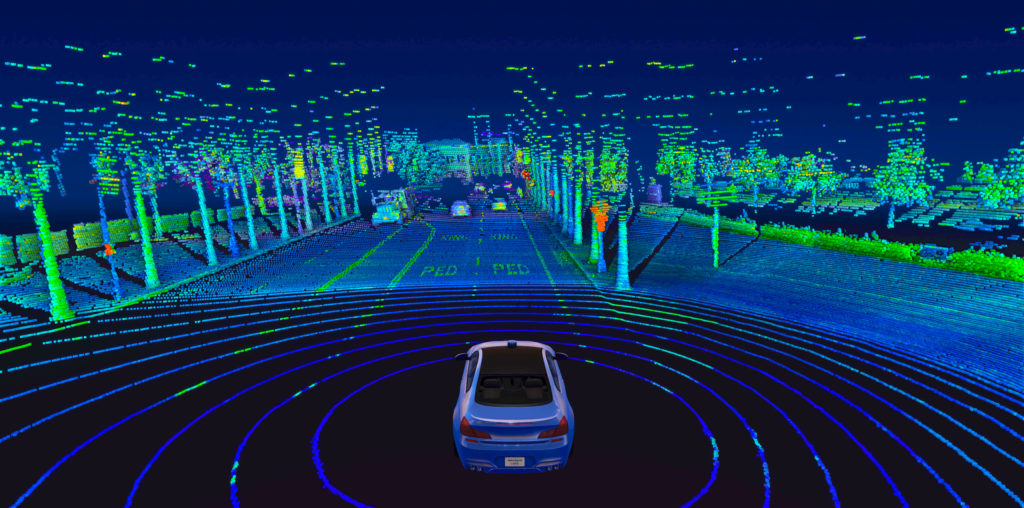
\includegraphics[width=0.45\textwidth,height=0.35\textheight]{map3d.jpg}$^\dag$
  \hfil
  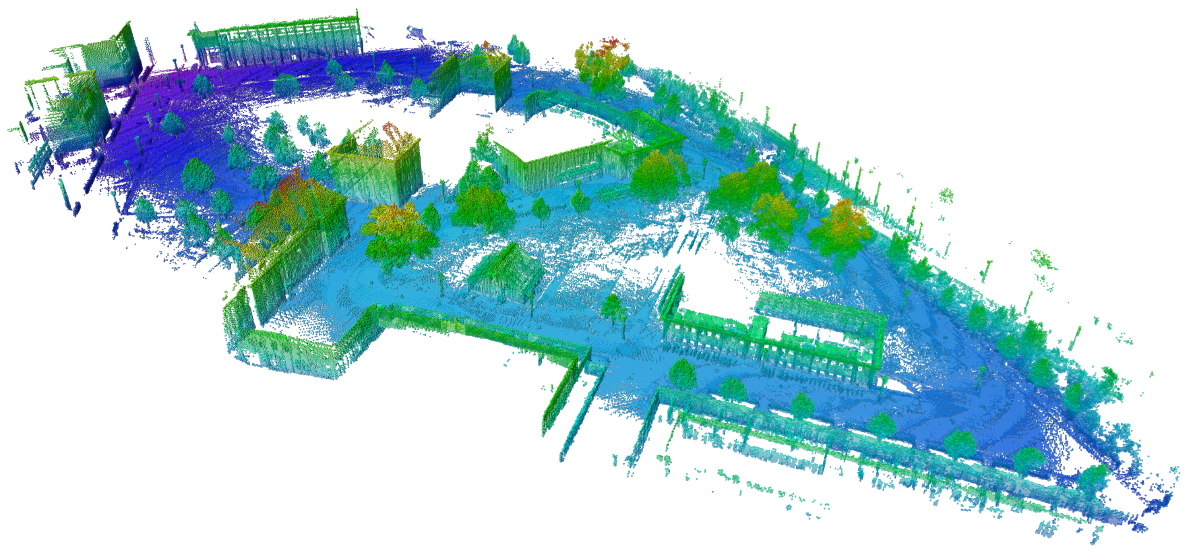
\includegraphics[width=0.45\textwidth,height=0.35\textheight]{map3d_2}$^\dag$
  \vspace{2pt}\\
  \bigskip % Vertical whitespace
  Es la construcción de un mapa del entorno, realizada por un robot, utilizando información espacial obtenida durante el paso del tiempo. [\citeauthor{Wallgrn2010} 2010]\\
  \bigskip % Vertical whitespace
  Fuentes de información:
  \begin{itemize}
  \item Escáners láser tipo LIDAR.
  \item Cámaras RGBD.
  \end{itemize}  

  \bigskip % Vertical whitespace
  
  \tiny La precisión del mapa debe corresponder con la precisión con la cual el robot necesita cumplir sus tareas.
  
  %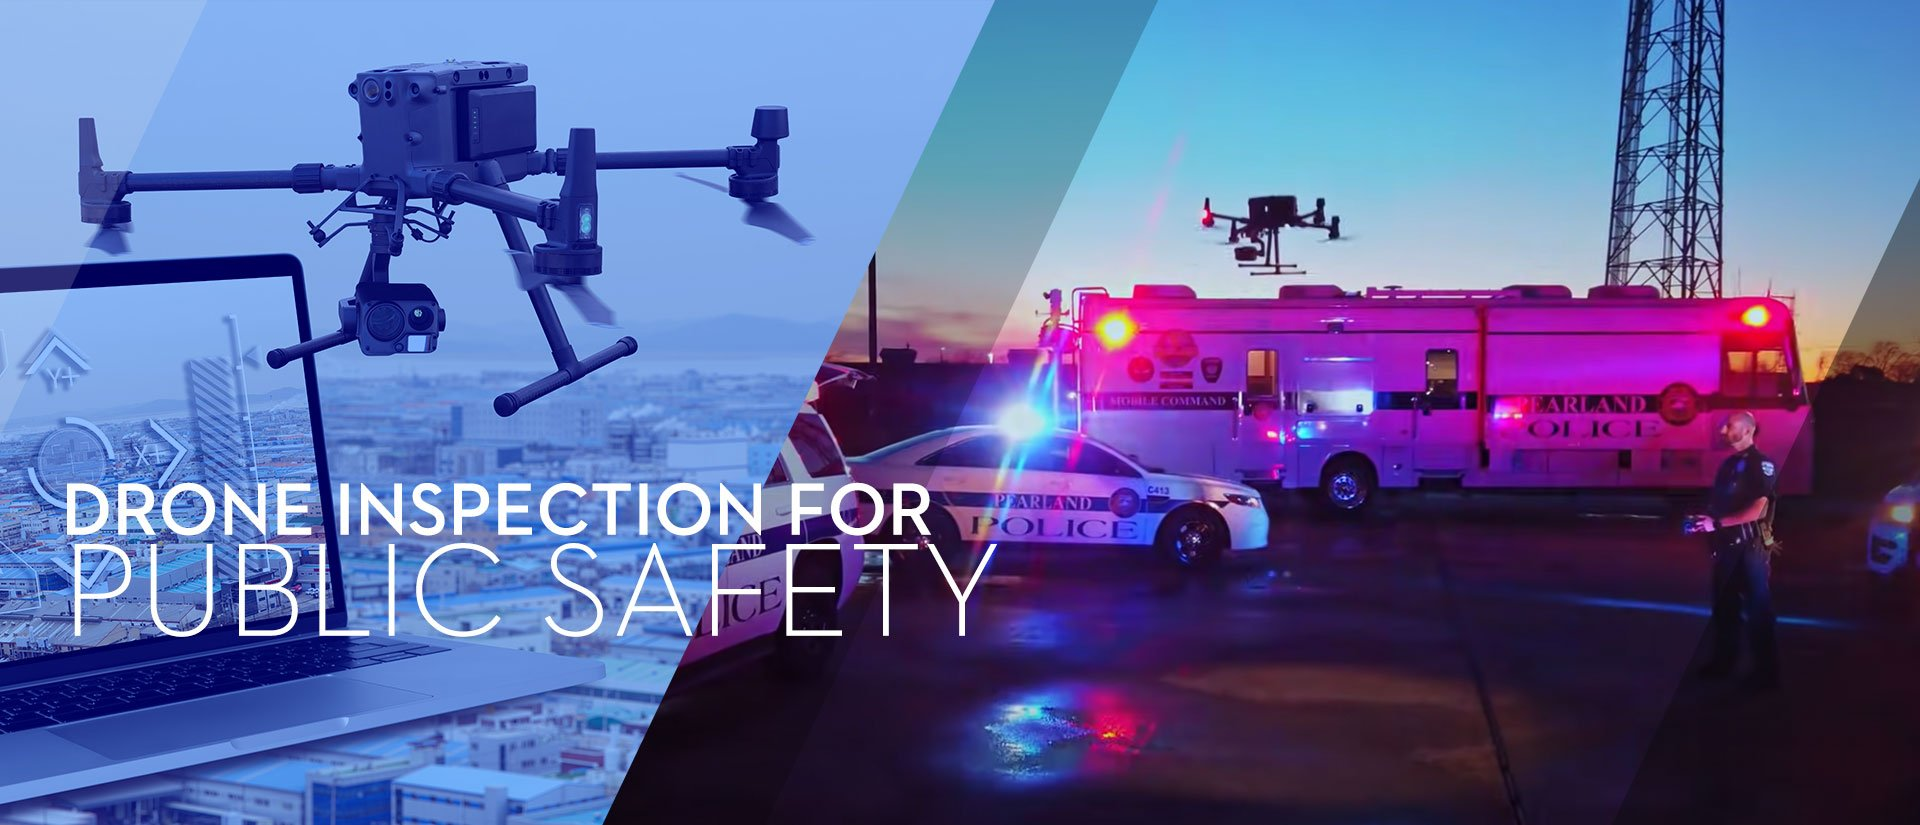
\includegraphics[width=0.45\textwidth,height=0.35\textheight]{DJI_B5}$^\dag$ 
  %\hfil
  %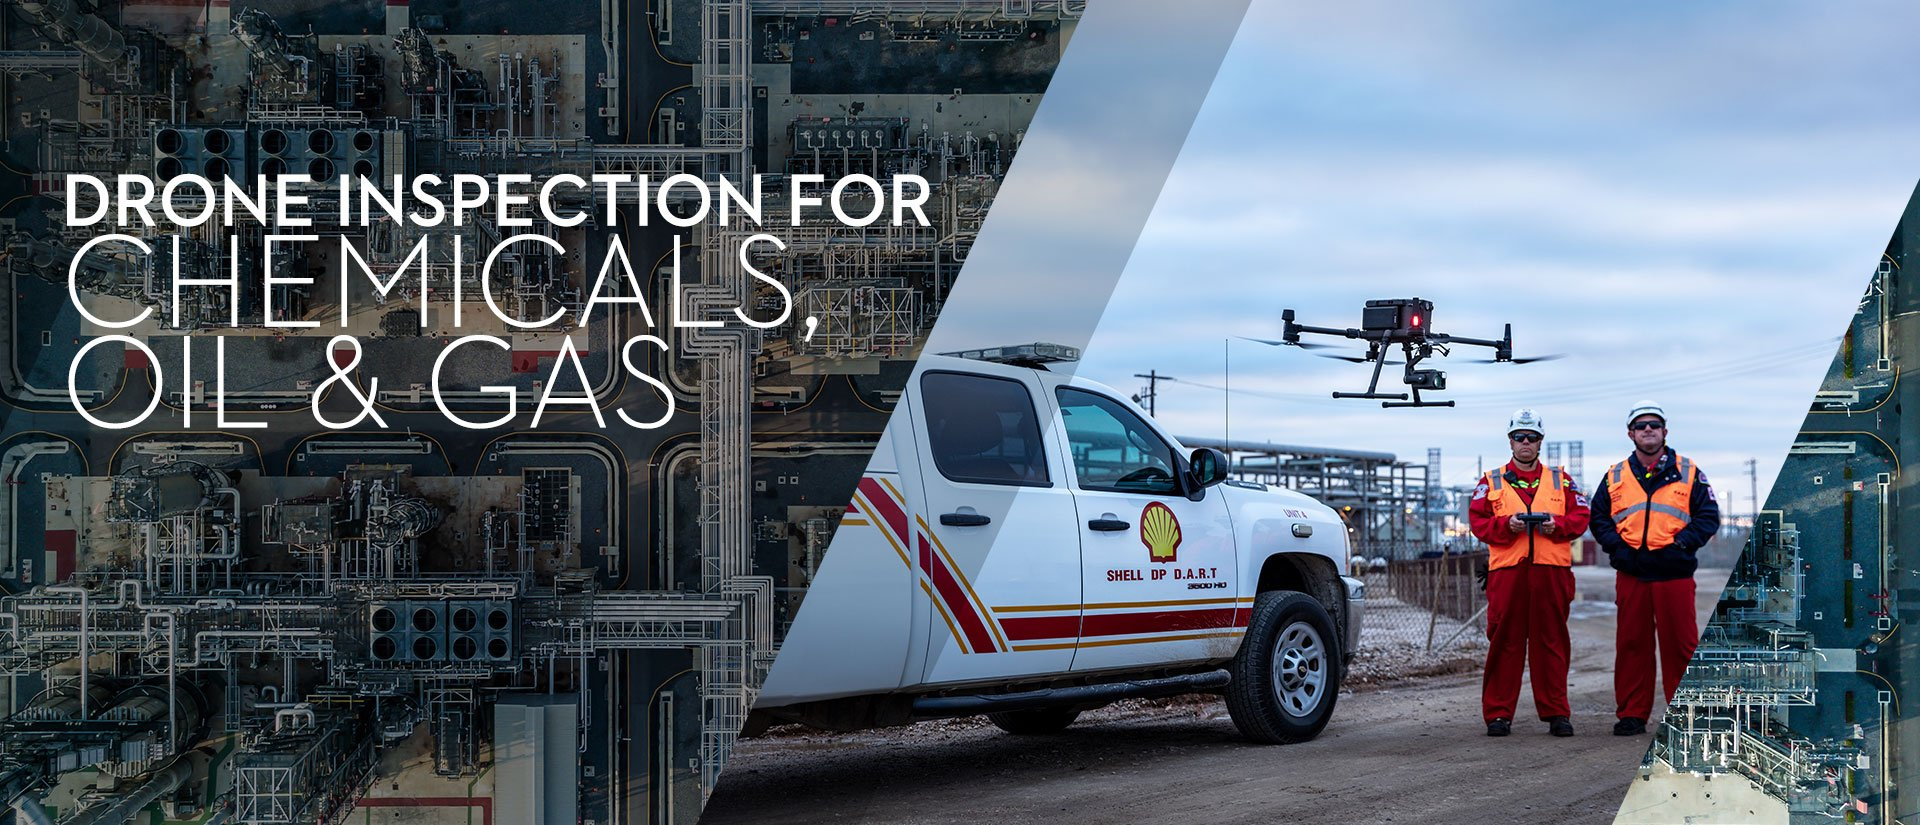
\includegraphics[width=0.45\textwidth,height=0.35\textheight]{DJI_B4}$^\dag$\\
  %\rule{0in}{1.2em}$^\dag$ \small Inspecciones con VANT basadas en los mejores casos de uso\\
  %\tiny \url{https://enterprise-insights.dji.com/blog/complete-guide-to-drone-inspections}
\end{frame}

\begin{frame}{Representación del Medio Ambiente - ¿Dónde estoy?}
  \bigskip % Vertical whitespace
  \centering
  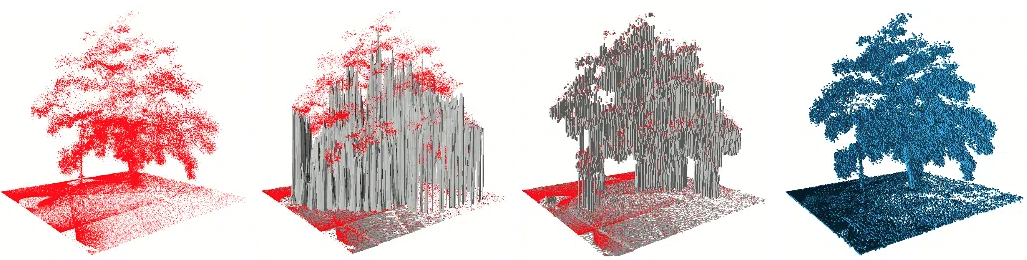
\includegraphics[width=1\textwidth,height=0.35\textheight]{img4}\footnotemark
  \vspace{2pt}\\
  \bigskip % Vertical whitespace
  
  \begin{itemize}
  \item Nube de puntos.
  \item Mapa de elevación.
  \item Superficies multi-nivel.
  \item Octomap (Octree).
  \item Hash Grid (HGrid).
  \end{itemize}
  \footnotetext{OctoMap: An Efficient Probabilistic 3D Mapping Framework Based on Octrees [\cite{hornung13auro}]}
  
\end{frame}

\begin{frame}{Representación del Medio Ambiente - ¿Dónde estoy?}

  \begin{itemize}
  \item Hash Grid (HGrid)
    \begin{itemize}
    \item Funciona bien para consultas de vecinos cercanos y búsquedas en un espacio tridimensional.
    \item Puede ser adaptativa a la densidad de objetos en diferentes áreas del espacio.
      \item Similar a la descomposición de un octree, pero su implementación con arrays, le permite una complejidad $O(1)$
    \item Puede requerir más memoria dependiendo de la resolución de la cuadrícula y la complejidad de la función hash.
    \end{itemize}
  \item Octomap (Octree).
    \begin{itemize}
    \item Tiende a ser más compacto en términos de almacenamiento de datos que algunas cuadrículas hash.
    \item Utiliza una estructura de árbol octree para representar la ocupación del espacio de manera eficiente.
    \item La actualización dinámica puede ser más desafiante y requerir técnicas adicionales.
    \end{itemize}
  \end{itemize}  
\end{frame}

\begin{frame}{Toma de decisiones - ¿A dónde voy?}
  %\centering
  \begin{figure}[h]
    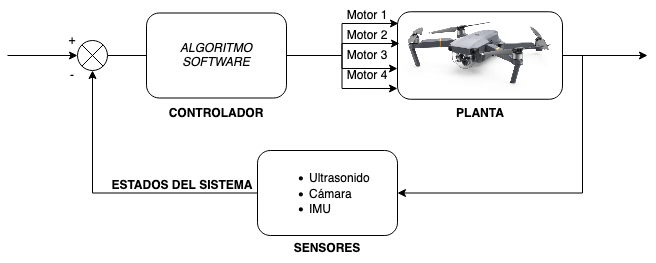
\includegraphics[width=0.65\textwidth]{control_drone.png}
    \caption{Diagrama control lazo cerrado VANT}
  \end{figure}
  \bigskip % Vertical whitespace
  \small Un sistema de control para un robot móvil autónomo opera en un entorno donde las condiciones están cambiando rápidamente. (considerando el problema de control instantáneo en una formulación clásica de teoría de control) \footnote{A robust layered control system for a mobile robot [\cite{brooks_robot}]}
  
\end{frame}

\begin{frame}{Arquitectura híbrida}
  \begin{minipage}{0.47\textwidth}
    
    \small El robot puede reaccionar de manera rápida a estímulos del entorno, al mismo tiempo que tiene la capacidad de planificar y tomar decisiones de alto nivel.
    
    \begin{itemize}
    \item Adaptable al lidiar con situaciones predecibles como imprevistas.
    \item Permite una respuesta rápida a estímulos del entorno.
    \item Optmiza el rendimiento del robot al gestionar las tareas simples y repetitivas, liberando recursos para tareas deliberativas más complejas.
    \item Es escalable.
    \end{itemize}
  \end{minipage}
  \hspace{0.2cm}
  \begin{minipage}{0.5\textwidth}
    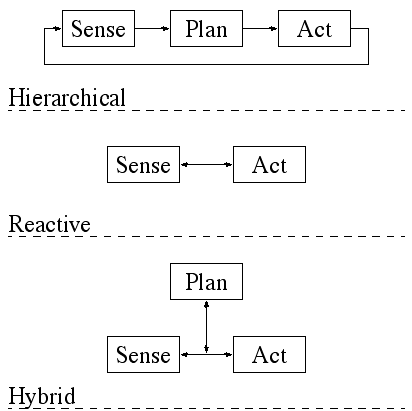
\includegraphics[width=0.8\textwidth]{architecture.png}$^\dag$\\
    \rule{0in}{1.2em}$^\dag$\scriptsize Ciclo Sense-Plan-Act \\
    \tiny \cite{murphy2000} %https://cs.brown.edu/people/tdean/courses/cs148/02/architectures.html#Murphy
  \end{minipage}
\end{frame}

\begin{frame}{Planificación de trayectoria - ¿Cómo llego hasta ahí?}
  \begin{minipage}{0.47\textwidth}

    El uso de heuristicas para encontrar soluciones óptimas, proporciona resultados computacionales eficientes. \footnote{A Survey of Trajectory Planning Techniques for Autonomous Systems [\cite{Mir2022}]} 
    \bigskip % Vertical whitespace
    \begin{itemize}
    \item Planificador de trayectoria global
      \begin{itemize}
      \item Búsqueda por grafos
      \end{itemize}
      \bigskip % Vertical whitespace
    \item Planificador de trayectoria local
      \begin{itemize}
      \item Campos de potencial artifical
      \item Algoritmos Bug
      \end{itemize}
    \end{itemize}
    \bigskip % Vertical whitespace
  \end{minipage}
  \hspace{0.2cm}
  \begin{minipage}{0.5\textwidth}
    \centering
    \animategraphics[loop,width=7cm]{10}{video-}{0}{46}
    \rule{0in}{1.2em}$^\dag$\scriptsize Aerial Navigation Development Environment.\\
    \tiny \url{https://www.youtube.com/watch?v=YrtLbCC49kg} 
  \end{minipage}
  
\end{frame}

\begin{frame}{Planificación de movimiento}
  \bigskip % Vertical whitespace
  \centering
  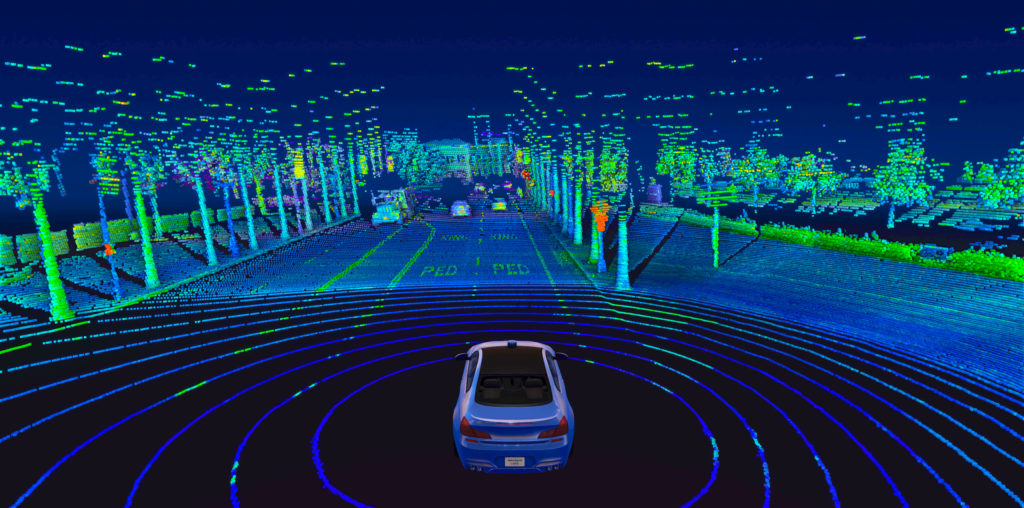
\includegraphics[width=0.45\textwidth,height=0.30\textheight]{map3d.jpg}$^\dag$
  \hfil
  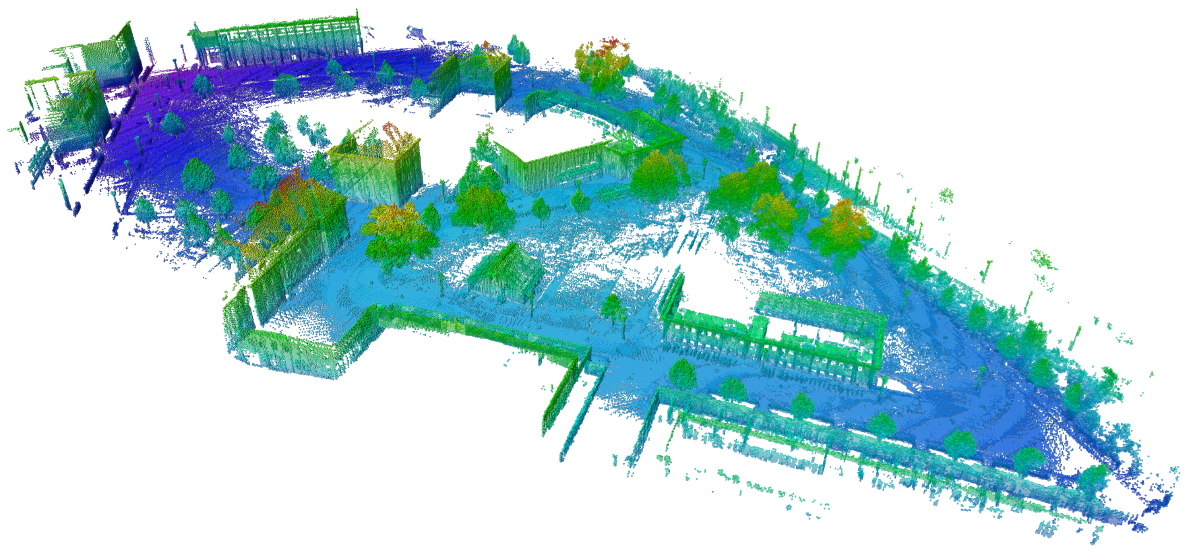
\includegraphics[width=0.45\textwidth,height=0.30\textheight]{map3d_2}$^\dag$
  \vspace{1pt}\\
  \bigskip % Vertical whitespace
  Indica a un robot como moverse de un punto a otro en su entorno. Implica la generación de trayectorias y movimientos que permiten a los robots cumplir sus tareas o alcanzar sus objetivos mientras evitan obstáculos \footnotemark.\\
  \bigskip % Vertical whitespace
  \addvspace{\medskipamount}
  \noindent
  \begin{tabularx}{\linewidth}{ @{} X X @{} }
    Por Grafos
    
    \begin{itemize}
    \item Grafos de visibilidad. 
    \item Diagramas de Voronoi.
    \item Descomposición por celdas.
    \item Consulta única (RRT)
    \item Consulta múltiple (PRM)
    \end{itemize} &

    Algoritmos
    
    \begin{itemize}
    \item BFS, DFS
    \item A*, D*
    \item Dijkstra
    \end{itemize}
  \end{tabularx}
  \footnotetext{Different Cell Decomposition Path Planning Methods for Unmanned Air Vehicles A Review [\cite{Debnath2020}]}
\end{frame}

\section{Exploración}

\begin{frame}
  \textbf{Exploración}\\
  \bigskip % Vertical whitespace
  Exploración es una tarea fundamental en robots autónomos. El objetivo es crear un mapa de un ambiente desconocido.\\
  \bigskip % Vertical whitespace
  \centering
  
\includegraphics[width=6cm]{exploracion}\\
  
  \begin{itemize}
  \item \textbf{Sensar} 
  \item \textbf{Creación Mapa} 
  \item \textbf{Localización en Mapa}
  \item \textbf{Exploración} Aumentar la base de conocimiento del Mapa
  \item \textbf{Planificación trayectoria} Trayectorias hacia nuevas fronteras 
  \item \textbf{Control} Ejecución de toma de decisiones y ejecución de trayectorias 
  \end{itemize}

  \pause \alert{El ciclo se repite hasta completar la exploración}
  
\end{frame}

\begin{frame}
  Enfoques de Exploración Por fronteras y NBVP
\end{frame}

\begin{frame}
  Fronteras
\end{frame}

\begin{frame}
  \begin{minipage}{0.47\textwidth}
    \textbf{Estrategia}
    \begin{itemize}
      %\item Exploración con algoritmos de baja complejidad computacional.
    \item \small Probabilistic Road-Map (Método a base de muestreos) \footnote{Survey of UAV motion planning [\cite{Quan2020}]}  
    \item \small RGB-D $\implies$ Voxels $\implies$ Octomap
      
    \item \small Exploración basada en fronteras \footnote{A frontier-based approach for autonomous exploration [\cite{613851}]}
    \item \small Estrategia basada en auto-ofertas (Método Húngaro) \footnote{Estrategia descentralizada para la exploración multi-robot, incluyendo restricciones en rango de comunicación [\cite{LEAL2013}]}
      
    \end{itemize}
  \end{minipage}
  \hspace{0.1cm}
  \begin{minipage}{0.5\textwidth}
    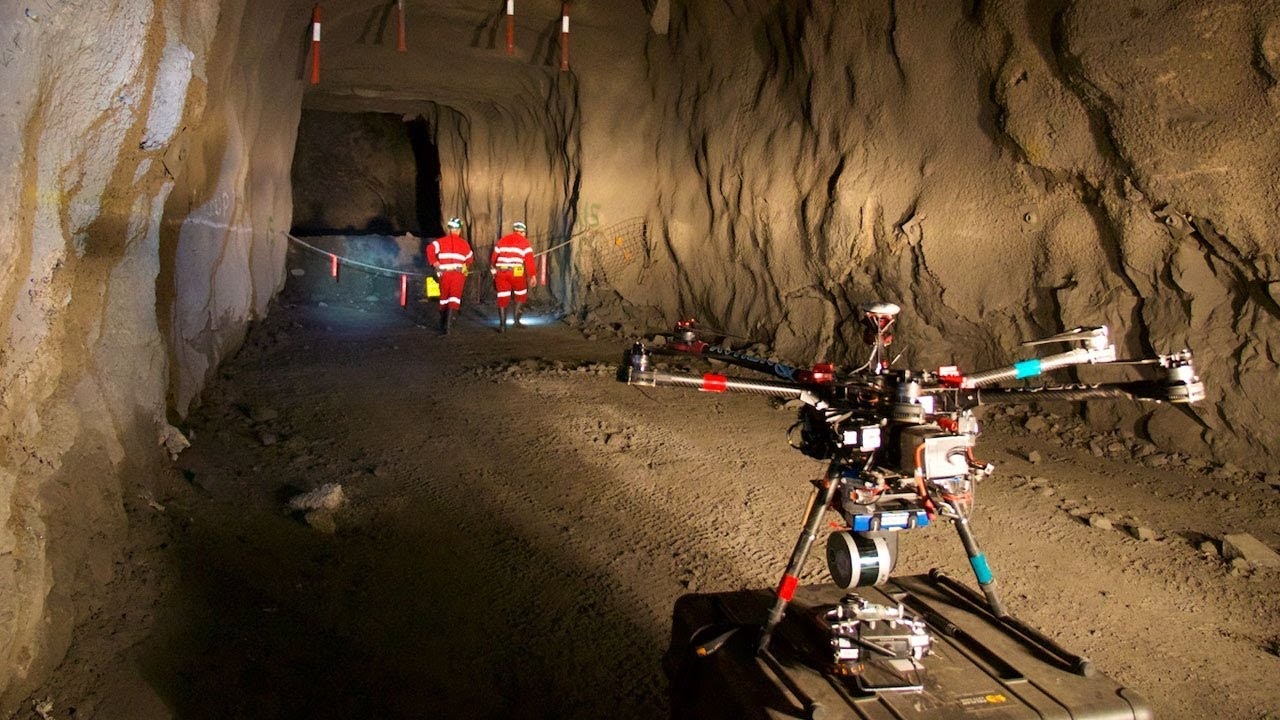
\includegraphics[width=\textwidth]{maxresdefault.jpg}$^\dag$\\
    \rule{0in}{1.2em}$^\dag$\scriptsize Ilustración Drone en Mina \\
    \tiny \url{https://dronevideos.com/} 
  \end{minipage}
  
\end{frame}

\begin{frame}

  \textbf{Estrategia} \footnote{Estrategia descentralizada para la exploración multi-robot, incluyendo restricciones en rango de comunicación [\cite{LEAL2013}]}\\
  
  \begin{minipage}{0.67\textwidth}
    \begin{itemize}
    \item[] \textcolor{teal}{Buscar que cada VANT se dirija hacia las fronteras más cercanas tratando de minimizar las distancias recorridas.}
      \bigskip % Vertical whitespace
    \item[] \textcolor{red}{Buscar la separación de los VANTS con la finalidad de minimizar el trabajo redundante y la interferencia entre ellos.}
      \bigskip % Vertical whitespace
    \item[] \textcolor{blue}{Mantener los VANTS en comunicación con los demás miembros del equipo actualizados y en caso de falla de algún VANT evitar que se pierda la información.}
    \end{itemize}
  \end{minipage}
  \hspace{0.6cm}
  \begin{minipage}{0.2\textwidth}
    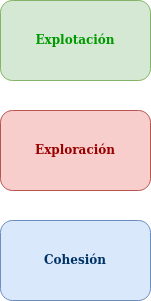
\includegraphics[width=1\textwidth]{estrategia}
  \end{minipage}
  
\end{frame}

\begin{frame}
  \textbf{Arquitectura}
  \begin{figure}
    \centering
    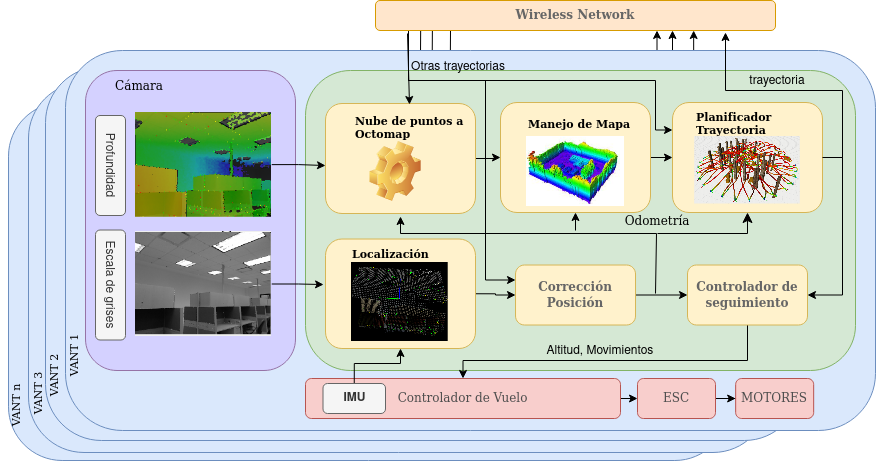
\includegraphics[width=15cm]{arquitectura}
  \end{figure}
\end{frame}

%\begin{frame}{Vehículos aéreos no tripulados (VANT)}
%  \bigskip % Vertical whitespace
%  \centering
%  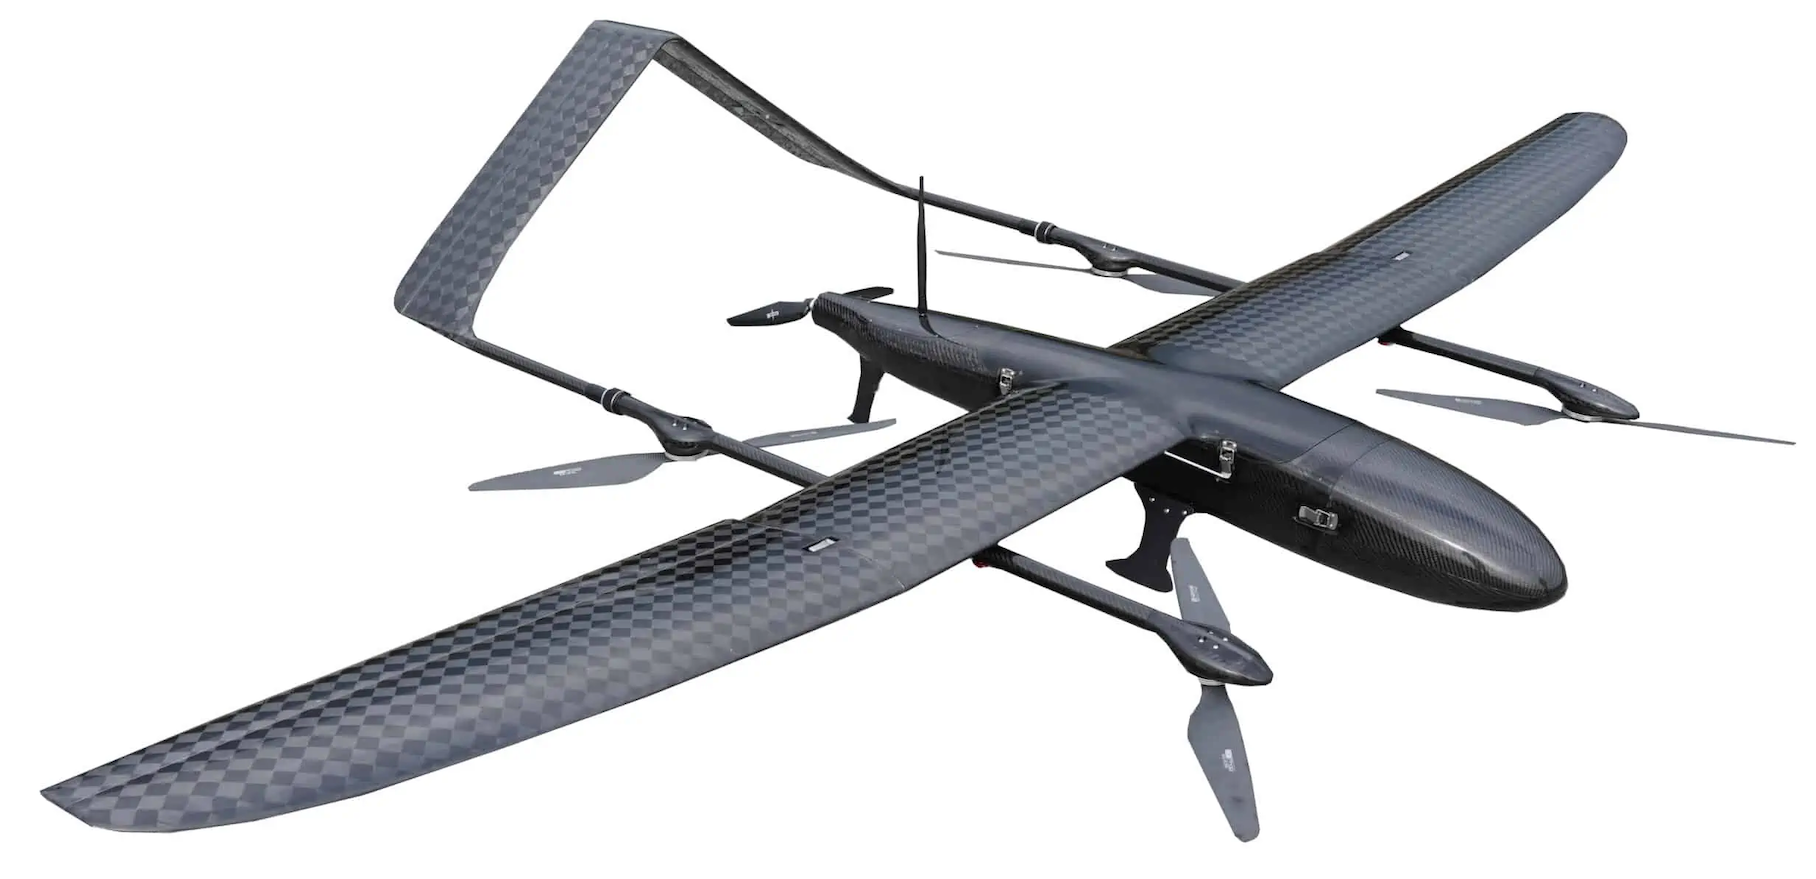
\includegraphics[width=0.45\textwidth,height=0.35\textheight]{img6}
%  \hfil
%  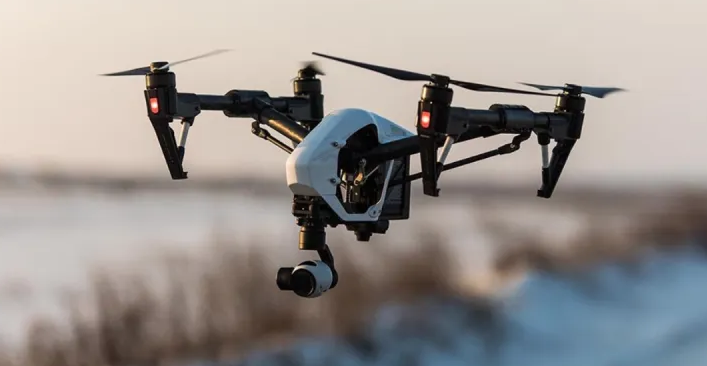
\includegraphics[width=0.45\textwidth,height=0.35\textheight]{img7}
%  \vspace{2pt}
%  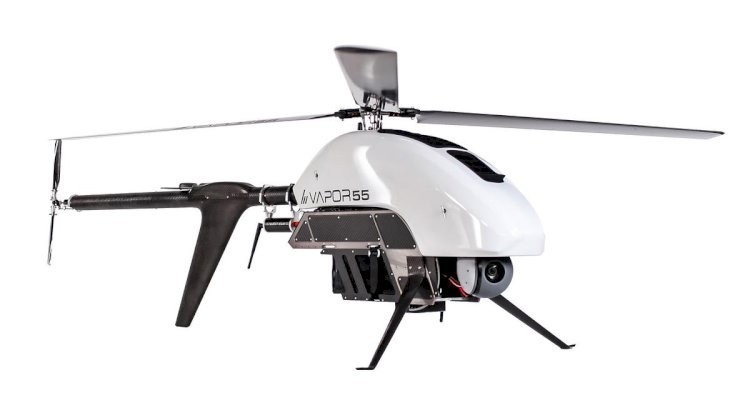
\includegraphics[width=0.45\textwidth,height=0.35\textheight]{img8.jpg}
%  \hfil
%  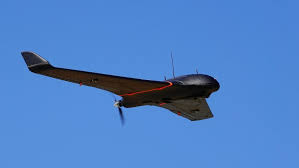
\includegraphics[width=0.45\textwidth,height=0.35\textheight]{img9.jpg}
%  \rule{0in}{1.2em} \small Clasificación VANTS \\
%  \tiny  Handbook of Unmanned Aerial Vehicles 2020
%\end{frame}

%\begin{frame}{Sistema autónomo VANT}
%  \begin{minipage}{0.47\textwidth}
    
%    \small Un sistema autónomo de un vehículo aéreo no tripulado consta de tres algoritmos.
    
%    \begin{itemize}
%    \item Generación de una representación del entorno.
%    \item Evasión de obstáculos.
%    \item Planificación de trayectorias.
%    \end{itemize}

%    \small La computadora embebida usado en un micro-VANT es de bajo rendimiento, pero su necesidad de autónomia sigue siendo la misma que un VANT de mayor tamaño.\\
%    Es necesario dotarlos de algoritmos de baja complejidad computacional.
    
%  \end{minipage}
%  \hspace{0.2cm}
%  \begin{minipage}{0.5\textwidth}
%    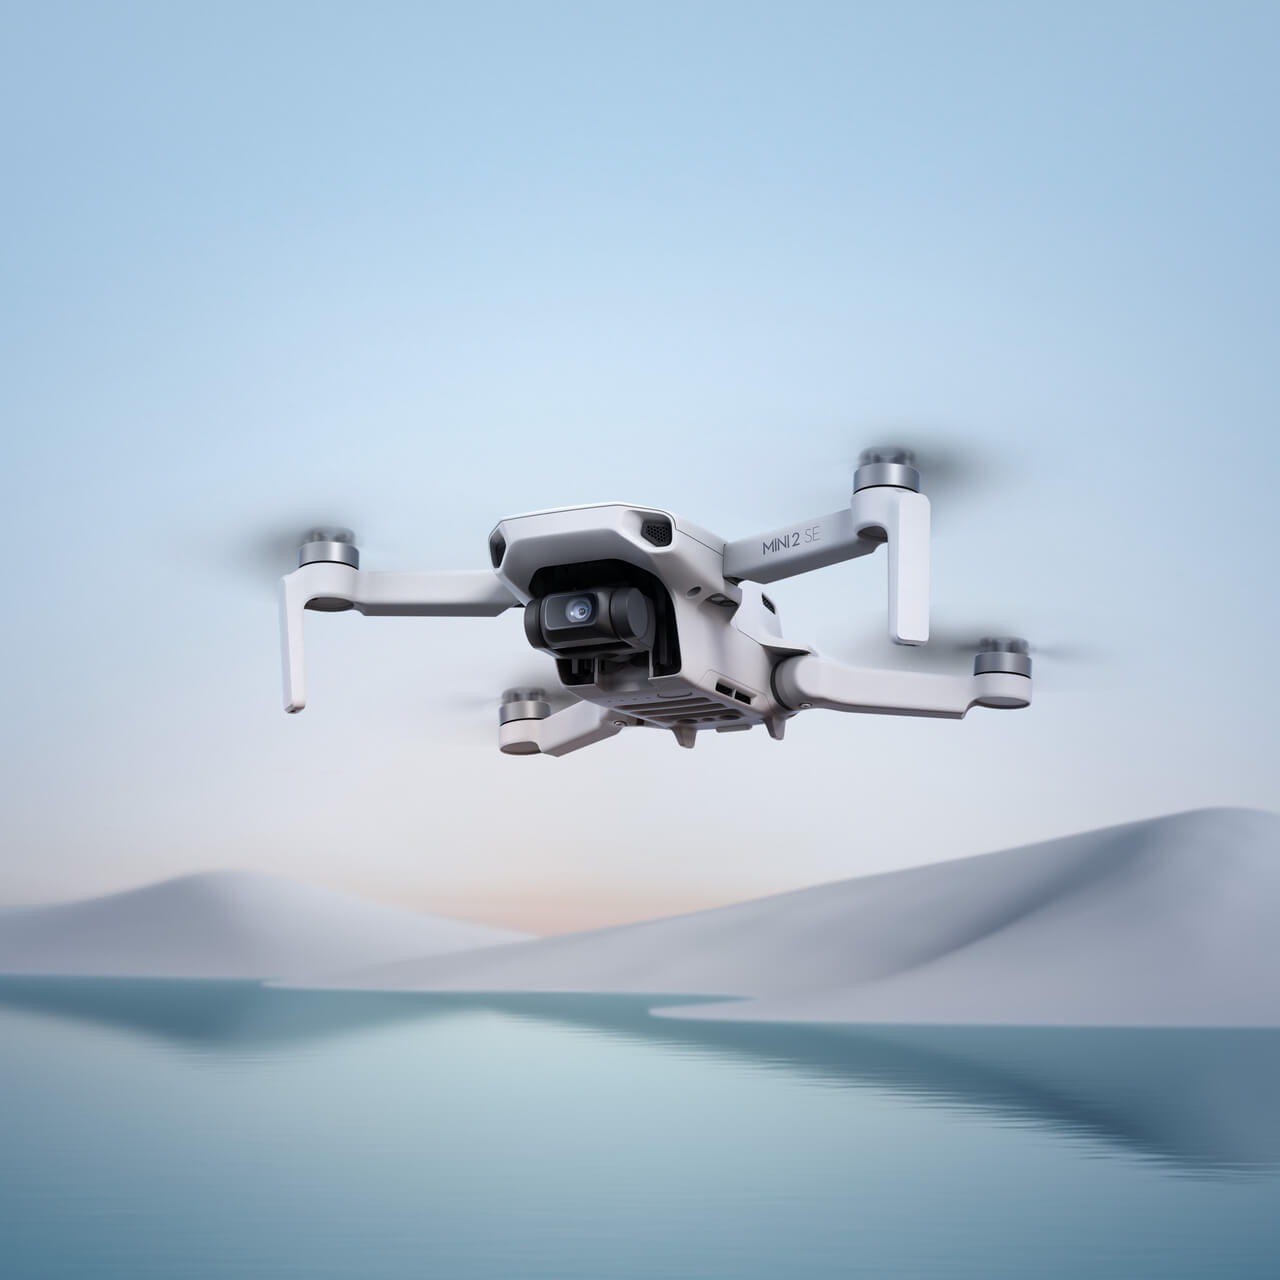
\includegraphics[width=\textwidth]{ultra.jpg}
%  \end{minipage}
%\end{frame}

\begin{frame}{Motivación del proyecto}
  \begin{minipage}{0.47\textwidth}

    \small La meta de este trabajo es la creación de una estrategia para la exploración de ambientes desconocidos de manera coordinada con múltiples vehículos aéreos no tripulados (VANTS).
    \bigskip % Vertical whitespace
    \begin{itemize}
    %\item Exploración con algoritmos de baja complejidad computacional.
    \item Búsqueda y rescate.
    \item Seguridad e Inspección
    \end{itemize}
  \end{minipage}
  \hspace{0.2cm}
  \begin{minipage}{0.5\textwidth}
    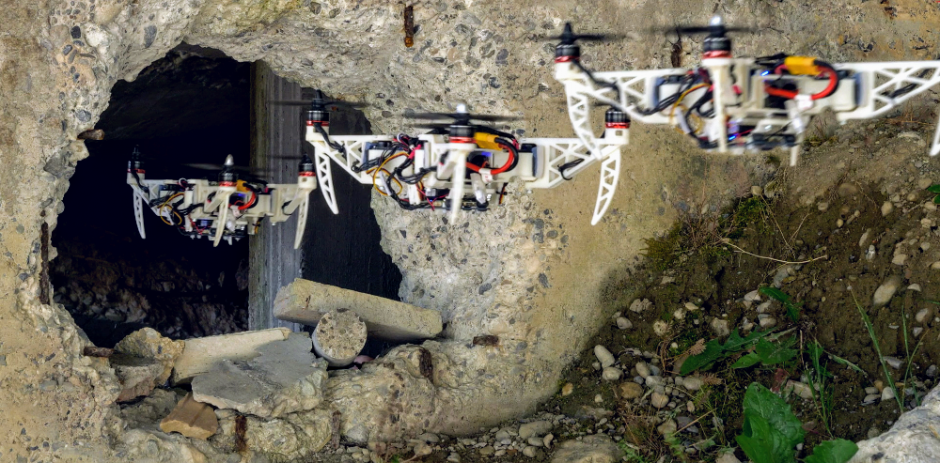
\includegraphics[width=\textwidth]{foldable-drone}$^\dag$\\
      \rule{0in}{1.2em}$^\dag$\scriptsize Foldable drone could aid search and rescue missions.\\
      \tiny \url{https://www.therobotreport.com/foldable-drone-could-aid-search-and-rescue-missions/} 
  \end{minipage}
\end{frame}

\section{Coordinación multi-VANT}
\begin{frame}{Coordinación multi-VANT}
Centralizada - Desentralizada
\end{frame}

%Explicar con el cronograma
\section{Simulación}
\begin{frame}{Simulación}
  \textbf{Robot Operating System (ROS)}\\
  \bigskip % Vertical whitespace
  \begin{itemize}
  \item Provee un conjunto de herramientas usadas por un robot (Sensores, actuadores, implementación diversos algoritmos)
  \item Framework de comunicación que permite interconectar las diferentes piezas del cerebro para hablar con otras lecturas de sensores.
  \end{itemize}
  \bigskip % Vertical whitespace
  En resumen ROS ayuda en descomponer software complejos en pequeñas piezas más manejables.
  
\end{frame}

\begin{frame}
  \begin{figure}
    \centering
    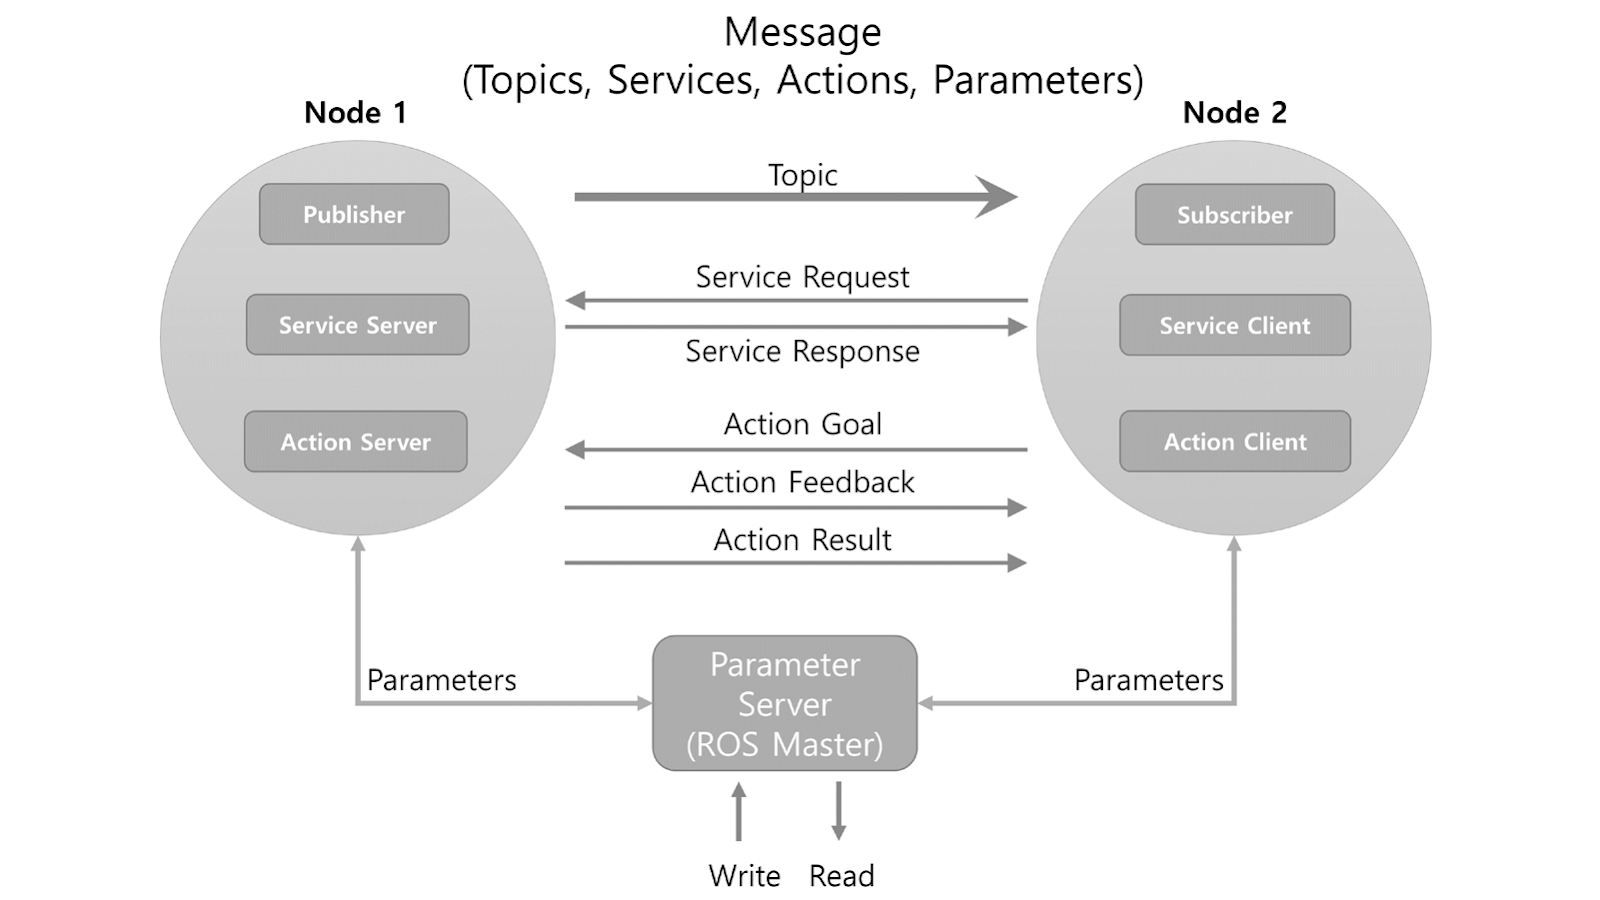
\includegraphics[width=0.75\textwidth]{ros_1}
  \end{figure}
\end{frame}

\begin{frame}
  \textbf{Simulador -  ROS Visualization (RVIZ)}
  \begin{figure}
    \centering
    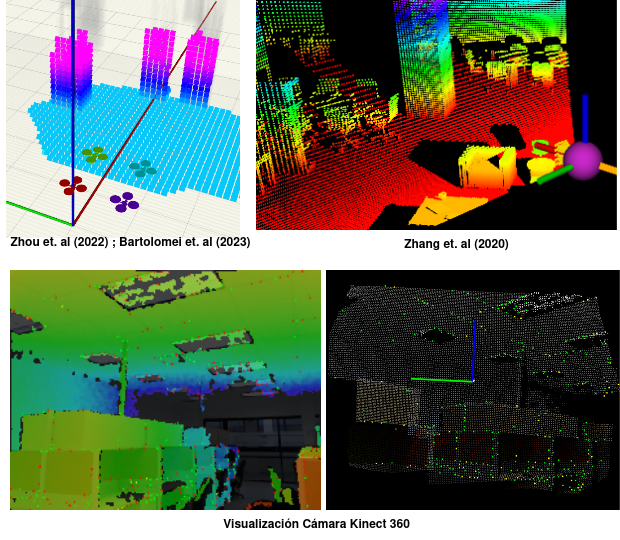
\includegraphics[width=0.57\textwidth]{visual}
  \end{figure}
\end{frame}

\begin{frame}
  El simulador dinámico \cite{RACER2022} \footnote{Rapid Collaborative Exploration With a Decentralized Multi-UAV System} utiliza la odometría de referencia de los VANTS, suponiendo que cada agente está equipado con una cámara de profundidad que mira hacia adelante cuya resolución es 640x480px y un campo de visión de 80°x60°. Las imágenes de profundidad se generan utilizando el proceso presentado en \cite{OMNI2022} \footnote{Omni-Swarm: A Decentralized Omnidirectional Visual–Inertial–UWB State Estimation System for Aerial Swarms} con un rango máximo de detección de 4.5 m.
  \bigskip % Vertical whitespace
  \begin{itemize}
  \item En tiempo necesario para completar la exploración del ambiente dado y la velocidad promedio de los VANTS durante cada experimento.
  \item Tasas de exploración para diferentes cantidades de VANTS en diversos ambientes.
  \end{itemize}
\end{frame}

\begin{frame}[allowframebreaks,noframenumbering]{Bibliografía}
  \tiny
  \bibliographystyle{abbrvnat}
  \bibliography{test}
\end{frame}

\end{document} 
